%% Modelo adaptado de abtex2-modelo-trabalho-academico.tex, v-1.8 laurocesar
%% Copyright 2012-2013 by abnTeX2 group at http://abntex2.googlecode.com/ 
%%
%% This work may be distributed and/or modified under the
%% conditions of the LaTeX Project Public License, either version 1.3
%% of this license or (at your option) any later version.
%% The latest version of this license is in
%%   http://www.latex-project.org/lppl.txt
%% and version 1.3 or later is part of all distributions of LaTeX
%% version 2005/12/01 or later.
%%
%% This work has the LPPL maintenance status `maintained'.
%% 
%% The Current Maintainer of this work is the abnTeX2 team, led
%% by Lauro César Araujo. Further information are available on 
%% http://abntex2.googlecode.com/

%%******************************************************
%%******************************************************
%% This work consists of the files:
%% abntex2-modelo-trabalho-academico-TCC-EngaEletrica.tex,
%% abntex2-modelo-include-comandos 
%% abntex2-modelo-references.bib
%%******************************************************
%%******************************************************

% ------------------------------------------------------------------------
% ------------------------------------------------------------------------
% abnTeX2: Modelo de Trabalho Academico (tese de doutorado, dissertacao de
% mestrado e trabalhos monograficos em geral) em conformidade com 
% ABNT NBR 14724:2011: Informacao e documentacao - Trabalhos academicos -
% Apresentacao
% ------------------------------------------------------------------------
% ------------------------------------------------------------------------

\documentclass[
	% -- opções da classe memoir --
	12pt,				% tamanho da fonte
	openright,			% capítulos começam em pág ímpar (insere página vazia caso preciso)
	onseside,
	%twoside,			% para impressão em verso e anverso. Oposto a oneside
	a4paper,			% tamanho do papel. 
	% -- opções da classe abntex2 --
	%chapter=TITLE,		% títulos de capítulos convertidos em letras maiúsculas
	%section=TITLE,		% títulos de seções convertidos em letras maiúsculas
	%subsection=TITLE,	% títulos de subseções convertidos em letras maiúsculas
	%subsubsection=TITLE,% títulos de subsubseções convertidos em letras maiúsculas
	% -- opções do pacote babel --
	english,			% idioma adicional para hifenização
	french,				% idioma adicional para hifenização
	spanish,			% idioma adicional para hifenização
	brazil,				% o último idioma é o principal do documento
	]{abntex2}


% ---
% PACOTES
% ---

% ---
% Pacotes fundamentais 
% ---
\usepackage{cmap}			% Mapear caracteres especiais no PDF
\usepackage{lmodern}			% Usa a fonte Latin Modern			
\usepackage[T1]{fontenc}		% Selecao de codigos de fonte.
\usepackage[utf8]{inputenc}		% Codificacao do documento (conversão automática dos acentos)
\usepackage{lastpage}			% Usado pela Ficha catalográfica
\usepackage{indentfirst}		           % Indenta o primeiro parágrafo de cada seção.
\usepackage{color}				% Controle das cores
\usepackage{graphicx}			% Inclusão de gráficos
% ---

\graphicspath{{images/}}

\usepackage{amsmath}
\usepackage{IEEEtrantools}
\usepackage{subfig}

% ---
% Pacotes adicionais, usados apenas no âmbito do Modelo Canônico do abnteX2
% ---
\usepackage{lipsum}			% para geração de dummy text
% ---

% ---
% Pacotes de citações
% ---
\usepackage[brazilian,hyperpageref]{backref}   % Paginas com as citações na bibl
\usepackage[alf]{abntex2cite}	                         % Citações padrão ABNT

% --- 
% CONFIGURAÇÕES DE PACOTES
% --- 

% ---
% Configurações do pacote backref
% Usado sem a opção hyperpageref de backref
\renewcommand{\backrefpagesname}{Citado na(s) página(s):~}
% Texto padrão antes do número das páginas
\renewcommand{\backref}{}
% Define os textos da citação
\renewcommand*{\backrefalt}[4]{
	\ifcase #1 %
		Nenhuma citação no texto.%
	\or
		Citado na página #2.%
	\else
		Citado #1 vezes nas páginas #2.%
	\fi}%
% ---


% ---
% Informações de dados para CAPA e FOLHA DE ROSTO
% ---
\titulo{Estudo Comparativo de Topologias de Microinversores Para Painéis Fotovoltaicos Conectados à Rede Elétrica}
\autor{Raul Henrique Santana}
\local{Belo Horizonte}
\data{2018}
\orientador{Prof. Pedro Francisco Donoso-Garcia}
%\coorientador{Prof. }
\instituicao{%
  Universidade Federal de Minas Gerais -- UFMG
  \par
  Escola de Engenharia
  \par
  Curso de Graduação em Engenharia Elétrica}
\tipotrabalho{Trabalho de Conclusão de Curso}

% O preambulo deve conter o tipo do trabalho, o objetivo, o nome da instituição e a área de concentração 
\preambulo{Monografia apresentada durante o Seminário dos Trabalhos de Conclusão do Curso de Graduação em Engenharia Elétrica da UFMG, como parte dos requisitos necessários à obtenção do título de Engenheiro Eletricista.}
% ---

% ---
% Configurações de aparência do PDF final

% alterando o aspecto da cor azul
\definecolor{blue}{RGB}{41,5,195}

% informações do PDF
\makeatletter
\hypersetup{
     	%pagebackref=true,
		pdftitle={\@title}, 
		pdfauthor={\@author},
    	pdfsubject={\imprimirpreambulo},
	    pdfcreator={LaTeX with abnTeX2},
		pdfkeywords={abnt}{latex}{abntex}{abntex2}{trabalho acadêmico}, 
		colorlinks=true,       	% false: boxed links; true: colored links
    	linkcolor=blue,          	           % color of internal links
    	citecolor=blue,        		% color of links to bibliography
    	filecolor=magenta,      		% color of file links
		urlcolor=blue,
		bookmarksdepth=4
}
\makeatother
% --- 

% --- 
% Espaçamentos entre linhas e parágrafos 
% --- 

% O tamanho do parágrafo é dado por:
\setlength{\parindent}{1.3cm}

% Controle do espaçamento entre um parágrafo e outro:
\setlength{\parskip}{0.2cm}  % tente também \onelineskip

% ---
% compila o indice
% ---
\makeindex
% ---

% ----
% Início do documento
% ----
\begin{document}

% Retira espaço extra obsoleto entre as frases.
\frenchspacing 

% ----------------------------------------------------------
% ELEMENTOS PRÉ-TEXTUAIS
% ----------------------------------------------------------
% \pretextual

% ---
% Capa
% ---
\imprimircapa
% ---

% ---
% Folha de rosto
% ---
\imprimirfolhaderosto
% ---

% ---
% Dedicatória
% ---
\begin{comment}


	\begin{dedicatoria}
	   \vspace*{\fill}
	   \centering
	   \noindent
	   \textit{ Este trabalho é dedicado às crianças adultas que,\\
	   quando pequenas, sonharam em se tornar cientistas.} \vspace*{\fill}
	\end{dedicatoria}

\end{comment}
% ---

% ---
% Agradecimentos
% ---

\begin{comment}

	\begin{agradecimentos}
	Os agradecimentos principais são direcionados à Gerald Weber, Miguel Frasson,
	Leslie H. Watter, Bruno Parente Lima, Flávio de Vasconcellos Corrêa, Otavio Real
	Salvador, Renato Machnievscz\footnote{Os nomes dos integrantes do primeiro
	projeto abn\TeX\ foram extraídos de
	\url{http://codigolivre.org.br/projects/abntex/}} e todos aqueles que
	contribuíram para que a produção de trabalhos acadêmicos conforme
	as normas ABNT com \LaTeX\ fosse possível.

	Agradecimentos especiais são direcionados ao Centro de Pesquisa em Arquitetura
	da Informação\footnote{\url{http://www.cpai.unb.br/}} da Universidade de
	Brasília (CPAI), ao grupo de usuários
	\emph{latex-br}\footnote{\url{http://groups.google.com/group/latex-br}} e aos
	novos voluntários do grupo
	\emph{\abnTeX}\footnote{\url{http://groups.google.com/group/abntex2} e
	\url{http://abntex2.googlecode.com/}}~que contribuíram e que ainda
	contribuirão para a evolução do \abnTeX.
	\end{agradecimentos}

\end{comment}
% ---

% ---
% Epígrafe
% ---
\begin{comment}


	\begin{epigrafe}
			\vspace*{\fill}
		\begin{flushright}
			\textit{``Não vos amoldeis às estruturas deste mundo, \\
			mas transformai-vos pela renovação da mente, \\
			a fim de distinguir qual é a vontade de Deus: \\
			o que é bom, o que Lhe é agradável, o que é perfeito.\\
			(Bíblia Sagrada, Romanos 12, 2)}
		\end{flushright}
	\end{epigrafe}

\end{comment}
% ---

% ---
% RESUMOS
% ---
% resumo em português
\begin{comment}

	\setlength{\absparsep}{18pt} % ajusta o espaçamento dos parágrafos do resumo
	\begin{resumo}
	Segundo a \citeonline[3.1-3.2]{NBR6028:2003}, o resumo deve ressaltar o
	objetivo, o método, os resultados e as conclusões do documento. A ordem e a extensão
	destes itens dependem do tipo de resumo (informativo ou indicativo) e do
	tratamento que cada item recebe no documento original. O resumo deve ser
	precedido da referência do documento, com exceção do resumo inserido no
	próprio documento. (\ldots) As palavras-chave devem figurar logo abaixo do
	resumo, antecedidas da expressão Palavras-chave:, separadas entre si por
	ponto e finalizadas também por ponto.

	\textbf{Palavras-chaves}: latex. abntex. editoração de texto.
	\end{resumo}

	% resumo em inglês
	\begin{resumo}[Abstract]
	\begin{otherlanguage*}{english}
		This is the english abstract.

		\vspace{\onelineskip}
	
		\noindent 
		\textbf{Key-words}: latex. abntex. text editoration.
	\end{otherlanguage*}
	\end{resumo}

\end{comment}

\begin{comment}
	% ---
	% inserir lista de ilustrações
	% ---
	\pdfbookmark[0]{\listfigurename}{lof}
	\listoffigures*
	%\cleardoublepage
	\clearpage
	% ---

	% ---
	% inserir lista de tabelas
	% ---
	\pdfbookmark[0]{\listtablename}{lot}
	\listoftables*
	%\cleardoublepage
	\clearpage
	% ---


	% ---
	% inserir lista de abreviaturas e siglas
	% ---
	\begin{siglas}
	%   \item[Fig.] Area of the $i^{th}$ component
	%   \item[456] Isto é um número
	%   \item[123] Isto é outro número
	%   \item[lauro cesar] este é o meu nome
		\item[CA] Corrente Contínua
		\item[CC] Corrente Contínua
	    \item[SCP] Sistema de condicionamento de Potência
	    \item[PCS] \textit{Power conditioning system}
		\item[MPPT] \textit{Maximum power point tracker}

	\end{siglas}

\end{comment}

% ---
\begin{comment}

	% ---
	% inserir lista de símbolos
	% ---
	\begin{simbolos}
	  \item[$ \Gamma $] Letra grega Gama
	  \item[$ \Lambda $] Lambda
	  \item[$ \zeta $] Letra grega minúscula zeta
	  \item[$ \in $] Pertence
	\end{simbolos}
	% ---

\end{comment}

% ---
% inserir o sumario
% ---
\pdfbookmark[0]{\contentsname}{toc}
\tableofcontents*
%\cleardoublepage
%\clearpage
% ---

% ----------------------------------------------------------
% ELEMENTOS TEXTUAIS
% ----------------------------------------------------------
\textual

% ----------------------------------------------------------
% Capítulo 1 - Introdução
% ----------------------------------------------------------
\chapter{Introdução}

\section{Motivação}

	A geração de energia elétrica no Brasil é fortemente caracterizada por um modelo geração centralizada e faz uso 
	do conceito de economias de escala \cite{MACHADO2016290}.
	Nesse modelo, plantas de grande porte geram toda a energia, que é transmitida e distribuída aos
	consumidores, ou seja, a energia é gerada de forma centralizada e posteriormente entregue ao destino final.
	%, para saber mais sobre isto veja \citeonline{mauriciomarinsmachado2014}. 
	Contudo, além dos riscos e danos ambientais ocasionados por tais centrais geradoras, com foco no cenário 
	brasileiro para a área alagada pelas usinas hidrelétricas, principal fonte de energia do país, 
	está associada à esta estrutura a necessidade de altos investimentos relacionados à distribuição da energia 
	gerada, tanto no condicionamento com a construção e manutenção de subestações quanto na transmissão.
	% quanto nas perdas que ocorrem durante a transmissão entre diferentes regiões.

	Nesse cenário, a geração distribuída de energia elétrica vem se mostrado cada vez mais uma alternativa viável.
	Uma rede de geração distribuída pode ser definida como um conjunto de fontes de energia conectadas diretamente 
	à rede de distribuição ou ao cliente \cite{ACKERMANN2001195}.

	Segundo a \textbf{ANEEL} (Agência Nacional de Energia Elétrica), desde 2012, com a vigência da solução normativa
	\href{http://www2.aneel.gov.br/cedoc/ren2012482.pdf}{Resolução Normativa ANEEL nº 482/2012}, é permitido ao 
	consumidor brasileiro gerar sua própria energia elétrica, se esta for proveniente de fontes renováveis ou cogeração qualificada.
	Uma maior adesão da população à GD tem como impactos esperados, além da diversificação da matriz energética nacional, 
	a redução do carregamento e das perdas nas redes, o adiamento de investimentos em expansão e distribuição e a redução 
	do impacto ambiental \cite{ANEEL_GD}.

	A principal vantagem na adesão ao sistema distribuído para o consumidor final é a capacidade de fornecer seu 
	excedente de produção à rede local, de modo a obter uma redução ainda maior do valor pago à concessionária de 
	energia no fim de cada mês.

	No conjunto de fontes renováveis, destaca-se a energia fotovoltaica, que converte a energia de raios solares em eletricidade 
	através de painéis fotovoltaicos (PV). Além de utilizar recurso abundante e não poluir durante a geração, sistemas geradores 
	fotovoltaicos necessitam de pouca manutenção e utilizam pouco espaço, podendo ser instalados nos tetos dos imóveis.
	Apesar disso, o custo de instalação destes geradores ainda é elevado e, portanto, é necessário maximizar a eficiência do 
	sistema. 	

	Um paiel fotovoltaico apresenta uma resposta não linear à incidencia solar sobre sua área e, para que seja extraído deste 
	a máxima potência possível devem ser utilizados algoritmos de rastreamento de ponto de máxima potência (MPPT). Aliados a 
	estes algortimos também se fazem necessários inversores de alto rendimento, responsáveis por condicionar a tensão 
	contínua fornecida pelos paineis em tensão alternada que pode ser injetada diretamente na rede elétrica.
	
%	Por executarem papel primordial na geração fotovoltaica e representarem cerca de 50\% de seu custo de implantação, a eficiência 
%	destes dispositivos  
 
	Por serem o elo de ligação entre o painel fotovoltaico e o sistema elétrico residencial e da concessionária, em sistemas \textit{on-grid} além de representarem uma parcela considerável do custo total da implantação do gerador os inversores apresentam 
	grande impacto na eficiência final do sistema de geração e, portanto, faz-se pertinente uma análise comparativa de custo e eficiência destes.


	A tensão disponibilizada por paineis fotovotaicos é geralmente de baixa amplitude, sendo necessária uma etapa de amplificação 
	entre o painel e a transformação do sinal contínuo em alternado. Esse estágio pode ser evitado em casos nos quais vários paineis 
	são conectados em série de modo que a tensão de saída do conjunto seja maior que a tensão de pico da rede. Esta configuração 
	é, entretanto, pouco usual em sistemas de baixa potência devido à necessidade de se garantir uma tensão mínima fornecida pelos 
	paineis. Sendo assim, as topologias mais comuns de inversores para sistemas fotovoltaicos utilizam um estágio elevador de tensão e um estágio inversor conectados em série \cite{LUIGIJUNIOR_ev_int}.

	Com o intuito de reduzir o custo e o espaço ocupado por inversores responsáveis por lidar com a energia gerada por uma série de paineis fotovoltaicos, vem sido estudada a utilização de microinversores \cite{Bouzguenda_smart_grid_inv}, inversores de menor potência, montados atrás de cada painel, pelo qual são responsáveis pela otimização da geração e pelo condicionamento da energia gerada. A principal vantagem na utilização de microinversores está no fato de estes isolarem os efeitos de sombreamento entre paineis \cite{Nezamuddin_des_eff_micro}.


	Os microinversores também são compostos, em geral, por dois estágios. O primeiro responsável por elevar a tensão fornecida pelo painel, além de sua operação no ponto de máxima potência e o segundo responsável por gerar a corrente alternada de modo a assegurar a correta conexão com a rede elétrica \cite{Nezamuddin_des_eff_micro}. Podem ser utilizadas, também, topologias integradas que buscam a simplificação e redução de componentes do circuito através da conexão direta entre os estágios \cite{LUIGI_int_top} \cite{LUIGIJUNIOR_ev_int}.

	
	É proposto nesse trabalho um estudo comparativo entre algumas topologias de microinversores para sistemas fotovoltaicos baseadas na estrutura CC-CC Ćuk. Serão estudados inversores com conversores Ćuk, Ćuk entrelaçado e Ćuk integrado com um inversor de onda completa, esse último proposto por \cite{LUIGI_int_top}.

	A utilização de conversores Ćuk se faz interessante devido ao fato de estes apresentam comportamentode fonte de corrente \cite{LUIGIJUNIOR_ev_int}, o que torna mais simples sua a conexão de sua saída à rede elétrica, que apresenta o comportamento de uma fonte de tensão, já que devem ser mantidos os níveis de tensão independente da corrente drenada. Isso elimina a necessidade de impedâncias em série entre o inversor e a rede elétrica, utilizadas para limitar a corrente de saída do inversor, as quais são necessárias quando este apresenta características de fonte de tensão. Além disso, o conversor Ćuk apresenta baixo ripple de corrente, o que resulta em baixas perdas e melhor eficiência na conversão \cite{Shawky_perform_anal}.



	A fonte de energia utilizada será um painel fotovoltaico com potência de aproximadamente 300W, será escolhido e implementado um algoritmo de MPPT e feita, também,  uma análise da distorção harmônica injetada por cada implementação.
%
%	Os circuitos propostos serão simulados no software \emph{PSIM}
%
%	A ferramenta principal desta iniciativa é o uso de simulação por %meio do PSIM.
%Portanto, a maior limitação deste trabalho será a avaliação de %dados reais, adicionalmente, não poderá ser feita uma análise %física dos sistema, o que inclui o peso do sistema
%montado, volume e temperatura durante a operação. Embora, para %comprovar resultados
%de forma efetiva, a montagem prática forneceria resultados %realistas, um software, como o
%PSIM, gera dados satisfatórios, pois foi construído especialmente %para analise de circuitos
%de eletrônica de potência. Consequentemente, como em vários artigos %citado nesta monografia, o Psim fornece resultados próximos à %realidade. Assim, para o objetivo de um
%estudante de graduação, simulações são suficientes para avaliar as %topologias de potência
%e o funcionamento que pode ser ligado à rede elétrica.
%

\section{Objetivo}

O objetivo princiapl deste TCC é o estudo, projeto, simulação e análise de um sistema de geração de energia elétrica composto por painel fotovoltaico e conversores CC-CC e CC-CA. 

As topologias de conversores que serão analisadas estão listadas a seguir e enquanto os conversores representam a coversão CC-CC, os inversores representam o estágio de

\begin{itemize}
	
	\item Conversor Ćuk convecional com Inversor em Ponte Completa
	\item Conversor Ćuk convecional com Inversor em Meia Ponte
	\item Conversor Ćuk Entrelaçado de 2 fases com Inversor em Ponte Completa
	\item Conversor Ćuk Entrelaçado de 2 fases com Inversor em Meia Ponte
	\item Conversor Ćuk integrado com Inversor em Ponte Completa
	\item Conversor Ćuk integrado com Inversor em Meia Ponte
	
\end{itemize}

\section{Estrutura Geral do Trabalho}

O capítulo 1 introduz o tema e o objeto de estudo, com uma breve explicação e contextualização do problema. No capítulo 2 é apresentado o estado da arte e apresetado o embasamento teórico necessário para o desenvolvimento do trabalho.

No capítulo 3 é descrita a metodologia utilizada, sendo o capítulo 5 dedicado à exposição dos resultados obtidos através desta. O sexto e útlimo capítulo é dedicado à discussão do resultado e às conclusões obtidas pelo estudo.

\chapter{Estado da Arte}

\section{Modelo do PV}

O circuito equivalente de células fotovoltaicas pode ser representado por uma fonte de corrente, como pode ser visto na figura ~\ref{fig:model_PV}. Este modelo é amplamente aceito e utilizado em trabalhos relacionados a energia fotovoltaica e seu comportamento do é descrito pelas equações~\ref{IPV_} a \ref{VOCPV}, nas quais $i_{pv}$ é a corrente e \emph{V} a tensão de saída da celula solar, respectivamente. 
$I_{ph}$ é a fotocorrente e $I_r$ a corrente reversa de saturação da célula, $R_s$ e $R_p$ são as resistências série e shunt, \emph{q} é a carga do elétrone $\eta$ é o fator de idealidade da junção p-n. \emph{k} é a constante de Boltzmann, \emph{T} representa a temperatura ambiente, em Kelvins e \emph{G} representa a densidade de potência da irradiação solar. 
$T_r$ é a temperatura nominal, em Kelvins (298K), $I_{sc}$ é a corrente de curto circuito em condições padrão de teste(\textit{STC}) ($T_r = 25ºC$ e $G =1kW/m^2$), $ \alpha $ é o coeficiente de temperatura, $I_rr$ é a corrente de saturação reversa em \textit{STC} e $E_g$ é o \textit{gap} de energia entre as bandas (1.1eV).
$V_{oc}$ é a tensão de circuito aberto das células, $N_s$ é o número de células por painel e $M_s$ é o número de painéis conectados em série \cite{PV-Teory}.
\begin{IEEEeqnarray} {c}
	i_{pv} = I_{ph} - I_r \left[ 
		\mathrm{e}^{q\left(\left(V+i_{pv}R_s\right)/\eta kT\right)} -1
		\right] - 
		\frac{V+i_{pv}R_s}{R_p} 
		\label{IPV_}\\
	 I_{ph} = \left[I_{SC} + \alpha \left(T - T_r \right)\right] \frac{G}{1000}
	 \label{IPH_}\\
	I_r = I_{rr} \left(\frac{T}{T_r}\right)^3 \mathrm{e}^{\left[\left(qE_g/\eta k\right) \left(\left(1/T_r \right)-\left(1/T\right)\right)\right]}
	\label{IR_}\\
	I_{rr} = \frac{I_{SC} - \left(V_{oc}/R_p\right)}{\mathrm{e}^{\left(qV_{oc}/\eta k T_r \right)} - 1 } 
	\label{IRR_}\\
	V_{pv} = V N_s M_s 
	\label{VPV_}\\
	V_{oc_{PV}} = V_{oc} N_s M_s
	\label{VOCPV}
\end{IEEEeqnarray}

\begin{figure}[h]%
	\begin{center}
		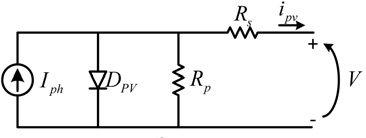
\includegraphics[width=0.55\linewidth]{pv_model}
		\caption{Circuito Equivalente de uma Célula Fotovoltaica \cite{PV-Teory}}
		\label{fig:model_PV}
	\end{center}
\end{figure}

A partir das equações ~\ref{IPV_},~\ref{IPH_},~\ref{IR_} e ~\ref{IRR_} é possível inferir a existência das relações entre a corrente de saída do painel fotovoltaico, sua temperatura e a irradiação solar. De fato, quanto maior a temperatura da célula, menor sua tensão de circuito aberto e, portanto, mais rápida sua variação de corrente. Já em relação à irradiação solar, quanto menor a magnitude desta, menor a corrente máxima da célula, relação clara ao analisar a equação~\ref{IPH_}.

Na figura~\ref{fig:iv_pv_} são apresentadas curvas I-V para diferentes valores de irradiação solar e temperatura de painel, para servirem de demonstração da influência dessas variáveis no comportamento do painel.

\begin{figure}%
	\centering
	\subfloat[]{{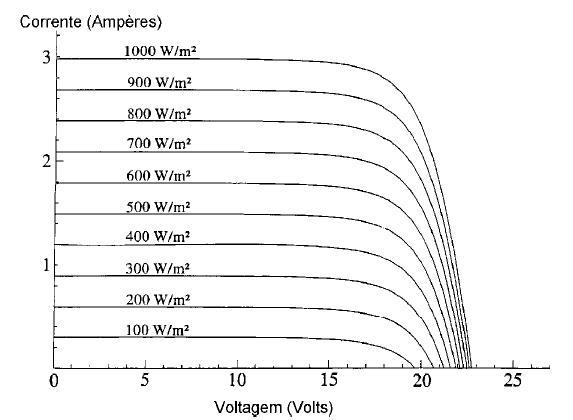
\includegraphics[width=0.45 \linewidth]{iv_PV} }}%
	\qquad
	\subfloat[]{{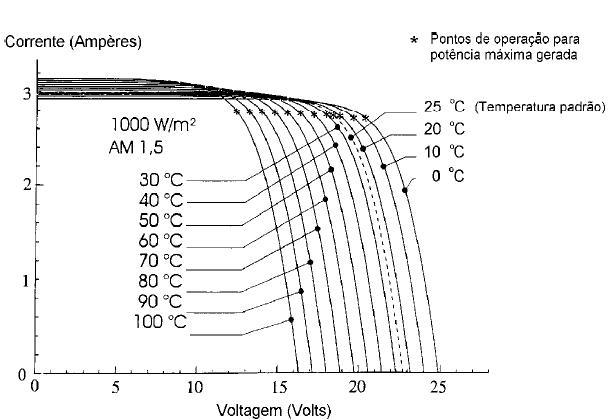
\includegraphics[width=0.45 \linewidth]{iv_pv2} }}%
	\caption{Curvas IxV de painel fotovoltaico para diferentes (a) irradiâncias e (b) temperaturas}%
	\label{fig:iv_pv_}%
\end{figure}


\section{Conversores Estáticos CC/CC}
%  BLABLABA SOBRE CONVERSORES ESTATICOS

\subsection{Conversor Ćuk Convencional}

Um conversor Ćuk é um conversor CC-CC baseado na transferência de energia capacitiva que é capaz de fornecer tensão maior ou menor que sua tensão de entrada, com polaridade invertida. Seu circuito pode ser visto na figura~\ref{fig:conv_cuk_circuit}. 

\begin{figure}[h]
	\begin{center}
		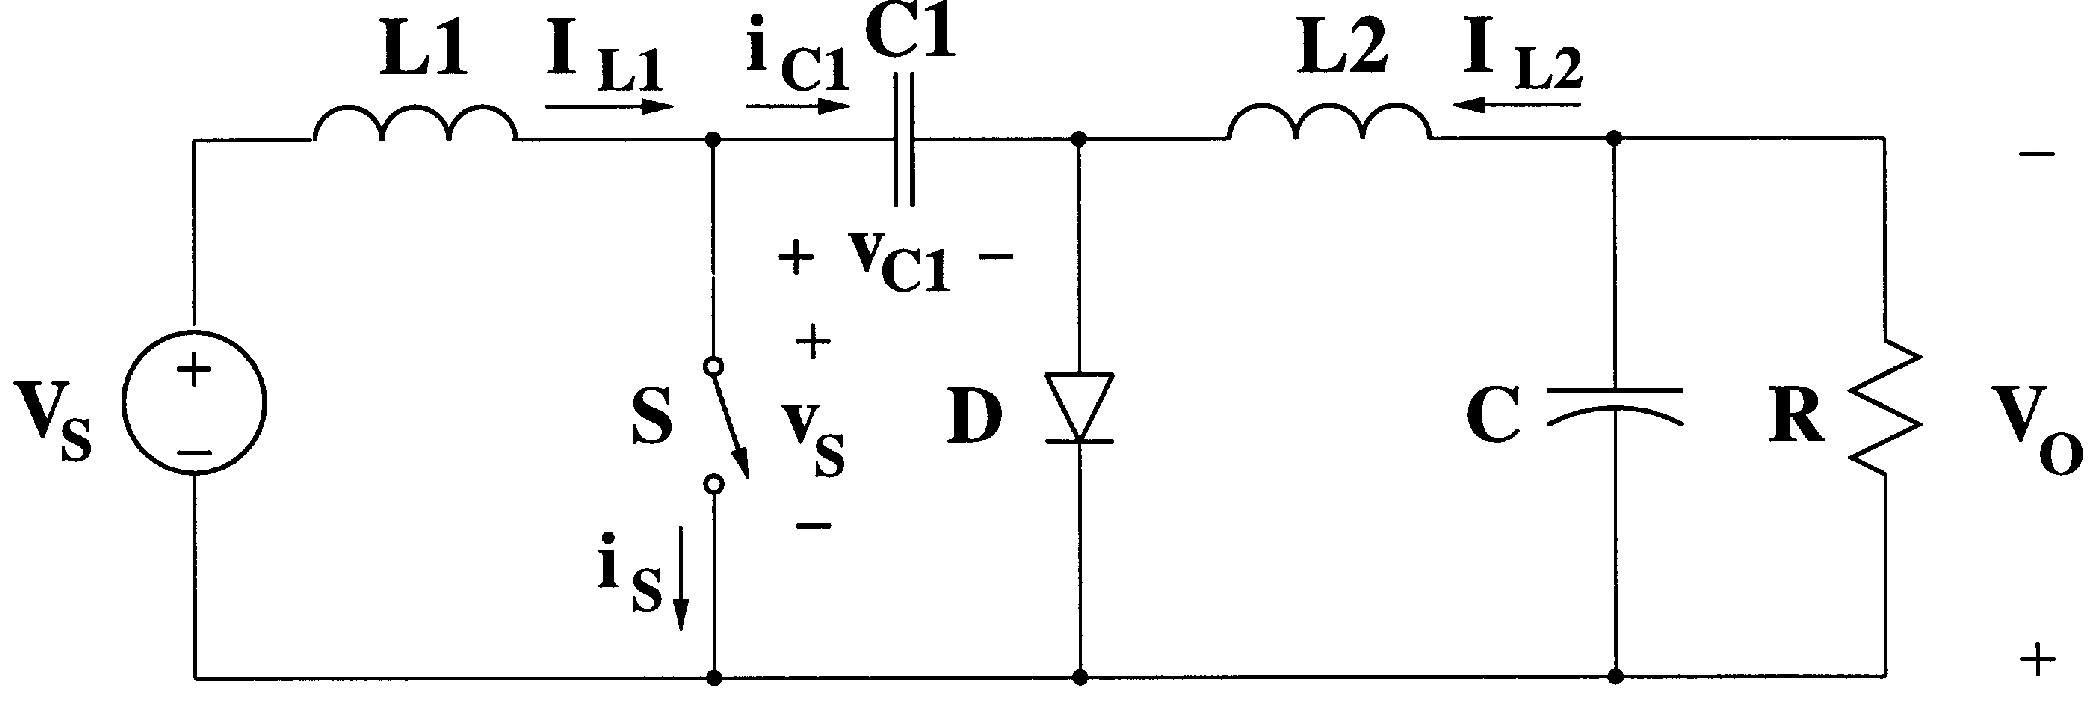
\includegraphics[width=0.55 \linewidth]{conv_cuk_circuit}
		\caption{Conversor Ćuk convencional \cite{RASHID_CUK}}
		\label{fig:conv_cuk_circuit}
	\end{center}
\end{figure}

Quando a chave \emph{S} está fechada (\textit{ON}), os indutores \emph{L1} e \emph{L2} são carregados pela tensão de entrada e capacitor \emph{C1}, respectivamente. O capacitor \emph{C1} polariza reversamente o diodo \emph{D} e descarrega fornecendo energia para a carga \emph{R}, o capacitor de filtro \emph{C} e o indutor de filtro \emph{L2}.
Com o transistor representado pela chave \emph{S} em estado aberto(\textit{OFF}), o indutor de entrada \emph{L1} carrega o capacitor de transferência de energia \emph{C1}. O diodo \emph{D} conduz as correntes de ambos \emph{L1} e \emph{L2} e, portanto, o indutor \emph{L2} descarrega fornecendo energia à carga \cite{RASHID_CUK} \cite{JOSEPH_2015_Intervealed_CUK}. 

A função de transferência CC desse conversor é dada pela equação~\ref{eq:trans_func_cuk_conv}, na qual \emph{d} é o ciclo de trabalho (\textit{duty cycle}), $V_s$ a tensão de entrada e $V_o$ a tensão de saída \cite{RASHID_CUK} \cite{JOSEPH_2018_Intervelead_cuk}.
\begin{equation}
	M_v = \frac{V_o}{V_s}= - \frac{d}{1-d}
	\label{eq:trans_func_cuk_conv}
\end{equation}
O conversor Ćuk opera em modo de condução contínua para $L1$ > $L_{b1}$ e $L2$ > $L_{b2}$ pelas equações~\ref{eq:cuk_conv_CCM_limits_l1} e ~\ref{eq:cuk_conv_CCM_limits_l2}.

O capacitor de filtro \emph{C} mínimo para uma certa tensão de ripple $V_r$ pode ser encontrado utilizando a equação~\ref{eq:rip_filt_conv_cuk}. Já a tensão de ripple no capacitor \emph{C1} pode ser estimada pela equação~\ref{eq:conv_cuk_rip_c1}.
\begin{IEEEeqnarray}{c}%
	L_{b1} = \frac{(1-d)R}{2df} \label{eq:cuk_conv_CCM_limits_l1}\\
	 L_{b2} = \frac{(1-d)R}{2f} \label{eq:cuk_conv_CCM_limits_l2} \\
	C_{min} = \frac{(1-d) V_o}{8 V_r L_2 f^2} \label{eq:rip_filt_conv_cuk}\\
	V_{r_{C1}} = \frac{dV_o}{C_1 R f} \label{eq:conv_cuk_rip_c1}
\end{IEEEeqnarray}

Nas equações~\ref{eq:cuk_conv_CCM_limits_l1} a \ref{eq:rip_filt_conv_cuk} $f$ é a frequência de chaveamento do transistor \emph{S}.

% Vale notar que a função de transferência da equação~\ref{eq:trans_func_cuk_conv} é igual à de um conversor \textit{Buck-Boost}.

% APRESENTA MODELO, PRINCIPIOS E INTRO AO PROJETO
\subsection{Conversor Ćuk Entrelaçado}

Um conversor cuk entrelaçado consiste de um capacitor, dois indutores, um transistor e um diodo para cada fase, além do capacitor de filtro que pode ser comum entre todas as fases. A figura~\ref{fig:interv_cuk_conv} apresenta o circuito de um conversor cuk entrelaçado de 2 fases.

Segundo \citeonline{JOSEPH_2015_Intervealed_CUK}, essa topologia tem o intuito de reduzir o ripple de corrente na entrada e reduzir o stress de chaveamento, sem sacrificar sua eficiência. Para tal, os transistores são ligados um por vez, por um período de ${T_{on}}/{2}$, e somente após passado um período ${T_{off}}/{2}$ do desligamento do transistor anterior. Isso é feito  utilizando-se a técnica de modulação por largura de pulso com desvio de fase, \emph{PSPWM}, do inglês \textit{Phase Shifted Pulse Width Modulation}.

O funcionamento do conversor cuk entrelaçado de 2 fases pode ser descrito em 3 modos~\cite{JOSEPH_2015_Intervealed_CUK}:
\begin{itemize}%
	\item Modo 1 ($t_0$-$t_1$): $S_1$ ligado e $S_2$ desligado;
	\item Modo 2 ($t_1$-$t_2$ e $t_3$-$t_4$): $S_1$ e $S_2$ desligados;
	\item Modo 3 ($t_2$-$t_3$): $S_1$ desligado e $S_2$ ligado.
\end{itemize}

No modo 1, ocorre a carga do indutor $L_{1a}$ e a descarga do indutor $L_{1b}$, que fornece energia ao capacitor $C_2$. Enquanto isso, o capacitor $C_1$ para a carga.

Assumindo uma variação linear na corrente dos indutores, a corrente de ripple para os indutores nesse modo pode ser calculada com as equações~\ref{eq:rip_interv_1} a \ref{eq:rip_interv_3}, nas quais $t_1$ é o tempo em que o transistor $S_1$ está ligado, $V_d$ a tensão de entrada e $V_{C_1}$ e $V_{C_2}$ a tensão nos capacitores $C_1$ e $C_2$, respectivamente.
\begin{IEEEeqnarray}{c}
	\Delta I_{L_{1a}} = \frac{t_1 V_d}{L_{1a}} \label{eq:rip_interv_1} \\
	\Delta I_{L_{1b}} = \frac{t_1 \left(V_{C_2} - V_d \right)}{L_{1b}} \label{eq:rip_interv_2} \\
	\Delta I_{L_2} = \frac{t_1 \left( V_{C_1} + V_o\right)}{L_2} \label{eq:rip_interv_3}
\end{IEEEeqnarray}

\begin{figure}[h]
	\begin{center}
		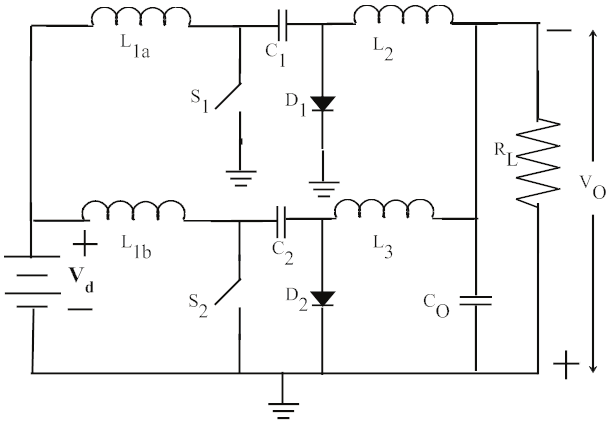
\includegraphics[width=0.55 \linewidth]{interv_cuk_circuit}
		\caption{Conversor Ćuk entrelaçado de 2 fases \cite{JOSEPH_2015_Intervealed_CUK}}
		\label{fig:interv_cuk_conv} 
	\end{center}
\end{figure}

Quando ambos os transistores estão desligados, ou seja, no modo 2, os indutores de entrada $L_{1a}$ e $L_{1b}$ são descarregados, fornecendo energia aos capacitores $C_1$ e $C_2$, respectivamente, de forma que, entre $t_1$ e $t_2$, $C_1$ carrega a energia que foi fornecida à carga no modo anterior, enquanto que entre $t_3$ e $t_4$, $C_2$ o faz. Além disso, os indutores $L_2$ e $L_3$ fornecem energia à carga e, portanto são descarregados.

Os ripples de corrente para os indutores nesse modo são encontrados utilizando as equações~\ref{eq:rip_interv_4} a \ref{eq:rip_interv_6}
\begin{IEEEeqnarray}{c}
	\Delta I_{L_{1a}} = \frac{t_2 \left(V_{C_1} - V_d\right)}{L_{1a}} \label{eq:rip_interv_4} \\
	\Delta I_{L_{1b}} = \frac{t_2 \left(V_{C_2} - V_d \right)}{L_{1b}}\label{eq:rip_interv_5} \\
	\Delta I_{L_2} = - \frac{t_2 V_o}{L_2} \label{eq:rip_interv_6}
\end{IEEEeqnarray}

No terceiro modo, com $S_2$ ligado, enquanto o indutor $L_{1b}$ continua sendo carregado, o indutor $L_{1a}$ é descarregado, fornecendo energia ao capacitor $C_1$. Por sua vez, o capacitor $C_2$ fornece energia à carga e aos componentes $L_3$, $C_o$.

Através das equações~\ref{eq:rip_interv_1}, \ref{eq:rip_interv_4},\ref{eq:rip_interv_3} e \ref{eq:rip_interv_6}, tem-se a equação da tensão de saída (\ref{eq:vo_interv}), onde $d = T_{on}/T$.
\begin{equation}
 V_o = - \frac{d \cdot V_d}{1 - d} \label{eq:vo_interv}
\end{equation}

\section{Conversores CC/CA - Inversores tipo fonte de tensão (\textit{VSI})}

A configuração básica de um inversor tipo fonte de tensão,\textit{VSI}, do inglês \textit{Voltage Source Inverter} é apresentada na figura~\ref{fig:vsi_3fas}. Para a obtenção de um inversor monofásico a única alteração necessária é remover um dos braços do circuito trifásico.

Havendo tensão na entrada do inversor, quando um transistor das semipontes superior ou inferior, nunca ao mesmo tempo, estiver em condução, a tensão CC aparecerá entre um par de condutores na saída alternada\cite{Pomilio_Cap_5}.

\begin{figure}[h]
	\begin{center}
		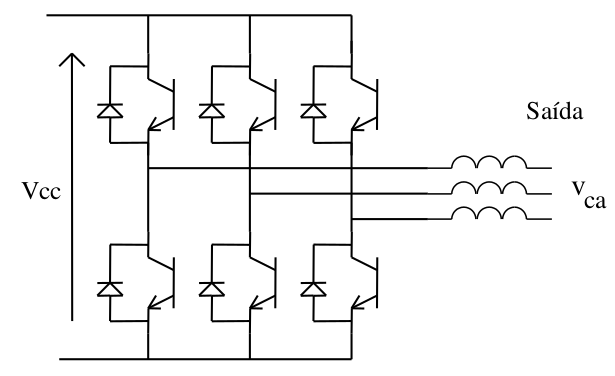
\includegraphics[width=0.55 \linewidth]{vsi_3fas}
		\caption{Inversor VSI trifásico \cite{Pomilio_Cap_5}}
		\label{fig:vsi_3fas}
	\end{center}
\end{figure}

\subsection{Inversor em Ponte Completa}
APRESENTA MODELO, PRINCIPIOS E INTRO AO PROJETO  E PWM
\subsection{Inversor em Meia Ponte}
APRESENTA MODELO, PRINCIPIOS E INTRO AO PROJETO, DIFERENÇAS AO PONTE COMPLETA E PWM

\section{Conversor Integrado (CC/CA)}
\subsection{Conversor Ćuk Integrado}
APRESENTA MODELO, PRINCIPIOS E INTRO AO PROJETO
\section{Rastreamento de máxima potência (\textit{MPPT})}

EXPLICA OQ É, PQ É NECESSÁRIO E SOBRE TECNICAS, PROVAVELMENTE SÓ UMA MESMO

\section{Modulação PWM}
FALAR SOBRE PWM SENOIDAL E PWM COM DESVIO DE fase

\section{PLL E FILTRO???????}
AVALIAR necessidade

\chapter{Metodologia}

\chapter{Resultados}

\chapter{Conclusão}

FALAR SOBRE  STATE OF THE ART EM INVERSORES X MICRONIVERSORES <---> FALAR SOBRE TOPOLOGIAS DE INVERSORES
DIFERENÇAS ENTRE MICRONIVERSORES E INVERSORES
VANTAGENS MICRONIVERSORES
MICRONIVERSORES NOS ULTIMOS anos

(microinvesores e inversores topologias, pq cuk?)
FALAR SOBRE TOPOLOGIA CUK (PQ ESCOLHER ESSA -> fonte de corrente?/ nova leva?)


	FALAR SOBRE TWO PANEL MICROINVERTERS TOPOLOGY




	% ajudam a reduzir a energia transmitida por longas distâncias e podem ser ligados diretamente à rede elétrica
	%  ou não, embora o primeiro caso seja mais usual, já que caso o produtor gerar mais energia que consome este 
	%  pode vender a energia excedente à concessionária de energia.
	% 
	% Em um sistema com geração distribuída, vários geradores de pequeno porte além da atual rede de geração centralizada. Estes produtores de energia de pequeno porte ajudam a reduzir a energia transmitida por longas distâncias e podem ser ligados diretamente à rede elétrica ou não, embora o primeiro caso seja mais usual, já que caso o produtor gerar mais energia que consome este pode vender a energia excedente à concessionária de energia.
	% 
	% Dentre as alternativas para a implantação deste sistema de geração distribuída estão as energias eólica e solar, principalmente. Entretanto a energia solar fotovoltaica tem chamado se destacado pela facilidade de operação e manutenção proporcionada, além do avanço nas tecnologias de células solares, com capacidade de conversão com eficiência de até 25,6\%, para o caso de células silício de junção única\cite{green2016solar}. 

	% 
	% Para a utilização de painéis fotovoltaicos conectados à rede elétrica de forma a possibilitar a venda do excedente de energia produzida à concessionária, é necessário a instalação de um inversor responsável pela conversão da tensão contínua fornecida pelos painéis em tensão alternada de 60Hz, correspondente à rede elétrica, além de um medidor especial que é capaz de mensurar a energia fornecida e a energia consumida pelo imóvel no qual os painéis estão instalados. 
	% Entretanto  para o caso em que todos os painéis forem ligados em série e conectados a um único inversor de alta potência o efeito de sombreamento de painéis se torna um problema considerável.
	% 
	% O efeito de sombreamento é causado por qualquer obstrução que faça com que os painéis não sejam irradiados com a mesma intensidade, de forma que as células que recebem menor radiação limitarão a corrente total que passa pela série de painéis. Além da possibilidade de dano às células, devido ao aumento da temperatura causado pela absorção de energia nos casos em que a corrente de saída do circuito é maior que a corrente da célula sombreada e o diodo desta seja polarizado reversamente \cite{7512858}, este efeito faz com que o potencial de geração dos painéis seja limitado pelos painéis sombreados.
	% 
	% Para contornar os problemas advindos tanto da ligação em série de diversos painéis fotovoltaicos quanto do uso de um único inversor de alta potência, podem ser utilizados inversores de baixa potência responsáveis pela conversão da energia gerada por um ou mais painéis e a conexão destes com a rede elétrica, os microinversores. Todavia, a utilização de um microniversor por painel pode resultar em um aumento do custo de implementação do sistema, já que, embora sejam necessários menos cabos com capacidade para altos valores de corrente serão necessários vários inversores eletrônicos em um sistema que anteriormente possuía apenas um, ainda que este seja maior e mais caro.
	% 
	% O objetivo deste trabalho é desenvolver um estudo comparativo de microniversores ligados à uma fonte primária, no caso um sistema fotovoltaico, à rede elétrica.
	% Para efetuar essa análise  serão estudadas as perdas em cada circuito, os algoritmos de MPPT, o desgaste e tempo de vida dos componentes e a viabilidade da montagem de um sistema fotovoltaico ligado à rede utilizando cada topologia.
	% Para finalizar o estudo os dados obtidos serão comparados de modo a evidenciar as características que diferenciam as topologias nos quesitos estudados. Além disso, será feita uma proposta de montagem da topologia com melhor desempenho.

% possa ser comparativo é analisar o custo de implementação, o tempo de vida útil e a eficiência energética de diferentes topologias de microniversores para conexão de painéis fotovoltaicos à rede elétrica. Estes parâmetros são importantes por estarem diretamente relacionados aos custos envolvidos na instalação e manutenção, além da capacidade de geração de um sistema fotovoltaico conectados à rede, variáveis de total interesse do consumidor final.


%, que deve optar por uma das várias combinações já presentes no mercado.

% A redução do custo  de compra de painéis fotovoltáicos tem levado ao aumento da produção de energia solar residencial.

%falar da visao ambiental crescente.
%Falar do custo baixo, falar do baixo rendimento dos paineis, explicitar vantagens do microniversor, em relação ao inversor.
%


\begin{comment}


  Os conversores multiníveis com tais topologias são aplicados em diversos sistemas. Dentre eles, estão os veículos elétricos e híbridos e aplicações de geração de energia a partir de painéis fotovoltáicos. No caso dos veículos elétricos, as baterias fornecem a tensão c.c. que é convertida em tensão c.a. para os motores de tração, sejam de indução ou síncronos. Para os painéis, a tensão c.c. gerada por eles é convertida para tensão c.a. com objetivo de fornecer energia elétrica a uma residência, por exemplo.

  Em ambos os casos, o recurso de fornecimento de energia é limitado e escasso. No caso dos painéis, ainda que a luz solar forneça bastante energia, o rendimento dos atuais painéis disponíveis no mercado é baixo. Dessa forma, o manejo dos recursos de tensão c.c. deve ser realizado com a máxima eficiência possível. Mesmo para casos em que o recurso não é escasso, como, por exemplo, metrôs e trens urbanos, o gasto de energia de tais aplicações é extremamente elevado e, portanto, um baixo rendimento torna os custos de operação muito elevados.

  O objetivo deste trabalho é analisar, dentre as configurações de conversores multiníveis, qual apresenta o melhor rendimento energético quando utilizados para tração elétrica. Tal parâmetro também será comparado com a complexidade da implementação da topologia, com os custos envolvidos na fabricação de tais conversores e com o comportamento frente às distorções harmônicas geradas.
  
\end{comment}


\begin{comment}

	\section{Informações gerais sobre este documento}
	Este documento e seu código-fonte são exemplos de referência de uso da classe
	\textsf{abntex2} e do pacote \textsf{abntex2cite}. O documento 
	exemplifica a elaboração de trabalho acadêmico (tese, dissertação e outros do
	gênero) produzido conforme a ABNT NBR 14724:2011 \emph{Informação e documentação
	- Trabalhos acadêmicos - Apresentação}.

	A expressão ``Modelo Canônico'' é utilizada para indicar que \abnTeX\ não é
	modelo específico de nenhuma universidade ou instituição, mas que implementa tão
	somente os requisitos das normas da ABNT. Uma lista completa das normas
	observadas pelo \abnTeX\ é apresentada em \citeonline{abntex2classe}.

	Sinta-se convidado a participar do projeto \abnTeX! Acesse o site do projeto em
	\url{http://abntex2.googlecode.com/}. Também fique livre para conhecer,
	estudar, alterar e redistribuir o trabalho do \abnTeX, desde que os arquivos
	modificados tenham seus nomes alterados e que os créditos sejam dados aos
	autores originais, nos termos da ``The \LaTeX\ Project Public
	License''\footnote{\url{http://www.latex-project.org/lppl.txt}}.

	Encorajamos que sejam realizadas customizações específicas deste exemplo para
	universidades e outras instituições --- como capas, folha de aprovação, etc.
	Porém, recomendamos que ao invés de se alterar diretamente os arquivos do
	\abnTeX, distribua-se arquivos com as respectivas customizações.
	Isso permite que futuras versões do \abnTeX~não se tornem automaticamente
	incompatíveis com as customizações promovidas. Consulte
	\citeonline{abntex2-wiki-como-customizar} par mais informações.

	Este documento deve ser utilizado como complemento dos manuais do \abnTeX\ 
	\cite{abntex2classe,abntex2cite,abntex2cite-alf} e da classe \textsf{memoir}
	\cite{memoir}. 

	Esperamos, sinceramente, que o \abnTeX\ aprimore a qualidade do trabalho que
	você produzirá, de modo que o principal esforço seja concentrado no principal:
	na contribuição científica.

	Equipe \abnTeX 

	Lauro César Araujo

\end{comment}

\begin{comment}
	% ---
	\section{Aliquam vestibulum fringilla lorem}
	% ---
	\lipsum[1]
	% ---

\end{comment}
% ----------------------------------------------------------
% Capitulo com exemplos de comandos inseridos de arquivo externo 
% ----------------------------------------------------------

%\include{abntex2-modelo-include-comandos}



%\begin{comment}
%
% \chapter{Revisão Bibliográfica}
%
%% \section{Histórico e Estado da Arte}
%
%%\chapter{Histórico e Estado da Arte}
%
%\section{Células e Painéis Fotovoltaicos}
%
%Em 1839, aos 19 anos de idade, o físico francês Edmond Becquerel descobriu o efeito fotovoltaico que foi inicialmente conhecido como efeito Becquerel \cite{Becquerel1839}. Este conduzia um experimento químico envolvendo uma célula eletrolítica composta por eletrodos metálicos de platina
%% e, posteriormente de prata,
% submersos em eletrólito, uma solução condutora de eletricidade \cite{111582}. Becquerel percebeu que ao iluminar um dos eletrodos, ocorria a circulação de corrente elétrica entre os terminais da célula. Uma figura do esquema da célula utilizada é mostrado na Figura~\ref{fig:BeqCell}, retirada de \citeonline{111582}.
%
%\begin{figure}[h]
%	\begin{center}
%		\includegraphics[width=0.5 \textwidth]{beqcell}
%		\caption{Diagrama da célula eletrolítica utilizada por Becquerel}
%		\label{fig:BeqCell}
%	\end{center}
%\end{figure}
%
%Segundo \citeonline{LINCOT2017381}, a primeira célula fotovoltaica operacional foi criada por C. Fritts \cite{Fritts01121883} em 1883 e posteriormente adotada por Werner von Siemens e J. Maxwell \cite{WSiemens1885}. Fritts inclusive foi responsável por implantar em um telhado de Nova Iorque o primeiro painel solar, composto por células fotovoltaicas ligadas entre si em série e/ou paralelo.
%% foi instalado em um telhado de Nova Iorque em 1884 por Fritts.
%
%Contudo, a primeira célula solar considerada eficiente, com eficiência de conversão maior que 5\%\footnote{Valor estipulado pelo departamento de gestão para credibilidade da indústria da Bell Labs}, foi apresentada somente em 1954 por \citeonline{doi:10.1063/1.1721711}, com capacidade de converter 6\% da energia irradiada sobre ela. A publicação desse artigo, inclusive, é amplamente considerada o nascimento da célula solar de silício \cite[p.~383]{LINCOT2017381}.
%
%Desde então foram feitos diversos avanços tecnológicos na área de conversão de energia fotovoltaica (de Arsenieto de Gálio), de forma a já serem possíveis células dotadas de uma única junção p-n com eficiência de até 28,8\%. %\footnote{Células de Arsenieto de Gálio (GaAs)}.
% Estes avanços também tornam factíveis módulos com células de silício, mais comuns no mercado devido ao menor custo de produção, tão eficientes quanto 23,8\%, segundo \citeonline{green2016solar}.
%
%Todavia, para a utilização da energia gerada pelos módulos fotovoltaicos seja para carregar baterias ou para a conexão com a rede elétrica se fazem necessários conversores eletrônicos de potência. O papel desses equipamentos eletrônicos é condicionar a tensão CC advinda dos módulos para a tensão de carregamento das baterias ou a tensão e frequência da rede(CA), de acordo com a característica do sistema. Além disso, também tem a função de proteger tanto os módulos quanto as baterias e a rede elétrica de qualquer anomalia que possa ocorrer, como curto-circuito, por exemplo.
%
%\section{Inversores e Microinversores solares}
%
%Para se aproveitar ao máximo e garantir a confiabilidade da energia gerada pelos módulos fotovoltaicos faz-se necessário conectá-los à conversores eletrônicos denominados inversores fotovoltaicos, também conhecidos como inversores solares.  Estes dispositivos eletrônicos podem ser divididos em dois tipos principais de acordo com tipo de utilização. Existem, portanto, inversores destinados para sistemas isolados (\textit{off grid}) e inversores destinados à ligação à rede elétrica (\textit{grid tie}).
%
%Nos projetos em que os inversores não serão conectados à rede de uma concessionária de energia são utilizados, geralmente, conversores CC/CC que,
%%ou CC/CA, sendo este último menos usual devido à incapacidade de alimentação em certos momentos do dia nos quais os painéis fornecem menos energia. Já o sistema para o primeiro caso deve,
%além de fornecer energia aos circuitos instalados, devem manter um banco da baterias carregado, proporcionando um estoque de energia disponível nos momentos em que os painéis não geram quantidade suficiente para suprir a demanda, durante a noite, por exemplo \cite{8378937,8357129,7439036}.
%
%Sistemas ligados à rede necessitam de um inversor eletrônico capaz de converter a tensão CC dos módulos em tensão CA, com frequência e amplitude devidamente alinhados a estes mesmos parâmetros no barramento de alimentação (rede da concessionária de energia). É muito importante, também, que estes dispositivos sejam capazes de oferecer proteção anti-ilhamento, para que nos momentos em que ocorra um problema na rede
%%  caso um problema ocorra na rede 
%elétrica e esta seja desligada, o inversor seja capaz de perceber esta alteração e cessar o fornecimento de energia à rede. Esta proteção tem o intuito de proteger tanto os equipamentos da rede elétrica quanto os trabalhadores que irão efetuar a manutenção da mesma.
%
%\subsection{Sistemas conectados à rede}
%%%%%%%%%%%%%%%%%%%%%%%%%%%%%%%%%%%%%%%%%%%%%%%%%%%%%%%%%
%%%%%%%%%%%%FALAR AQUI SOBRE AS POSSIVEIS MONTAGENS DOS PAINEIS --- SERIE, PARALELO, MISTO, CARALHO A 4
%%%%%%%%%%%%%%%%%%%%%%%%%%%%%%%%%%%%%%%%%%%%%%%%%%%%%%%%%
%
%Os sistemas de condicionamento de potência, SCP ou PCS, do inglês \textit{power conditioning systems}, podem ser catalogados em três categorias: \textbf{SCPs centrais}, \textbf{SCPs série} e \textbf{SCPs integrados ao módulo} \cite{Kwon2009}.
%
%Como o próprio nome já diz, SCPs centrais são aqueles ligados ao barramento CC formado pela diferença de potencial criada pela associação dos módulos fotovoltaicos.%, seja em série quanto em paralelo,
%Esta estrutura de módulos apresenta tanto um alto valor de tensão quanto capacidade para alta potência, de forma que os inversores utilizados nestes sistemas também apresentam estas características. Além de problemas estruturais como a necessidade de cabos de alta tensão CC entre o conversor e os painéis, esta configuração ainda apresenta eficiência relativamente baixa devido ao efeito de sombreamento parcial e ao desequilíbrio entre os arrays de painéis conectados em paralelo \apud[p.~410]{Kwon2009}{Zhang2006}.
%
%Já no sistema de condicionamento de potência série, cada inversor é responsável por um conjunto de painéis conectados entre série, que chamamos de \textit{array}. Estes inversores são conectados em paralelo entre si e conseguem extinguir o problema do desequilíbrio entre conjuntos de painéis em paralelo
%%, já que todos estão ligados em série
%. Todavia, apesar de reduzir os problemas com sombreamento relatados para os SCPs centrais, estes continuam presentes.
%
%Por fim, sistemas integrados ao módulo têm um inversor dedicado por módulo, de forma a extinguir o problema de sombreamento parcial. Além disso, cada módulo tem seu próprio MPPT (\textit{maximum power point tracker}), responsável por fazer com que o sistema trabalhe sempre na melhor condição possível, ou próximo dessa, em relação à potência desenvolvida. Com isso, em questão de eficiência, esta configuração apresenta resultados melhores que as demais. Entretanto, possui custo de implantação maior que as demais, já que são necessários tantos inversores quanto o número de módulos presentes na instalação.
%
%Na Figura~\ref{fig:SCPs} estão apresentadas as categorias de SCP, nas quais:
%\begin{enumerate}[label=(\alph*)]
%\item SCP central
%\item SCPs série
%\item SCPs integradas aos módulos
%\end{enumerate}
%
%
%\begin{figure}[!ht]
%	\begin{center}
%		\includegraphics[width=0.7 \textwidth]{pcsKinds}
%		\caption{Os três tipos de SCP}
%		\label{fig:SCPs}
%	\end{center}
%\end{figure}
%
%
%\subsection{Inversores conectados à rede elétrica}
%
%Segundo \citeonline{Mallwitz2010}, em 1991 chegaram ao mercado os primeiros inversores fotovoltaicos produzidos em série. Estes apresentavam rendimento de cerca de 90\% e faixa de tensão CC de entrada muito estreita. Esta última característica limitava a quantidade de módulos que poderiam ser ligados ao dispositivo e, portanto, a capacidade de geração por inversor.
%% E, em 1995 foi lançado o primeiro inversor para sistemas série, chamado "Sunny Boy". 
%
%Uma segunda geração de inversores começou a ser produzida em 2004. Entre as melhorias em relação à primeira geração pode-se destacar principalmente a capacidade de resfriamento do circuito. Apresentou eficiência máxima de 98\%, em laboratório ainda em 2006, ainda segundo \citeonline{Mallwitz2010}
%
%Já em 2007 era apresentada ao mercado a terceira geração de inversores fotovoltaicos. Com potência nominal acima de 5kW e uma nova topologia, os inversores dessa família diferem consideravelmente das famílias anteriores, tanto em potência nominal quanto em complexidade. Em 2008 foi demonstrada eficiência de 99\% em montagens laboratoriais para inversores dessa família \apud[p.~2]{Mallwitz2010}{zacharias2009}.
%
%% A Figura~\ref{fig:milestones}, retirada de \cite{Mallwitz2010}
%
%\subsection{Microniversores conectados à rede elétrica}
%
%Um microinversor nada mais é que um inversor de menor potência. Um microinversor solar é usualmente projetado para trabalhar conectado a apenas um módulo fotovoltaico, embora hajam propostas de microniversores de potências mais altas para conexão de até 4 painéis\cite{Kwon2009}. É, portanto, essencialmente um SCP integrado ao módulo.
%
%Apesar de ter seu conceito concebido desde o início da utilização de inversores fotovoltaicos, os custos de produção associados à montagem dos inversores fizeram com que este modelo reduzido fosse preterido por apresentar maior custo por Watt suportado. As principais vantagens em relação ao modelo mais usual estão tanto na manutenção mais simples, barata e menos frequente quanto no aumento da produção de energia, devido ao fato de que cada painel funciona no ponto ótimo por ter um MPPT dedicado. 
%
%Um sistema projetado com microinversores é capaz de atingir um custo de produção de energia até 25\% menor que um sistema mais convencional, com inversores de grande porte. Entretanto o custo da produção ainda é superior ao patamar para  energia residencial não subsidiada, de 3 dólares \apud[p.~469]{Dong2018}{Elasser2010}.
%
%Módulos fotovoltaicos modernos apresentam potência máxima de produção, raramente atendida, na faixa de 225W a 275W. Devido a este fato, microniversores dedicados a esses painéis geralmente apresentam potência por volta dos 220W. Por serem projetados para trabalhar com potências baixas foram desenvolvidas topologias de circuito que eliminam a necessidade da utilização de transformadores grandes e capacitores eletrolíticos, responsáveis por aumentar o espaço físico necessário para montar o equipamento e a reduzir a vida útil do circuito, já que esses componentes apresentam um ciclo de vida mais curto que os demais. Para mais sobre o tempo de vida útil de capacitores eletrolíticos consulte \citeonline{Zhao2010}.
%
%A principal desvantagem destes inversores, entretanto é o custo inicial do equipamento. Apesar de tornar desnecessário a utilização de cabos para altas correntes e de gerar mais energia com o mesmo número de painéis, o número de inversores utilizados é maior. %Dessa forma o investimento inicial não é tão atrativo.
%
%%%%%%%%%%%%%%%%%%%%%%%%%%%%%%%%%%%%%%%%%%%%%%%%%%%%%%%%
%%% FALAR AQUI DOS MICRO INVERSORES
%% VANTAGENS - DESVANTAGENS - DIFERENÇAS
%%%%%%%%%%%%%%%%%%%%%%%%%%%%%%%%%%%%%%%%%%%%%%%%%%%%%%%%
%
%% \section{Topologias de Microinversores}
%
%
%\chapter{Fundamentação Teórica}
%
%Inversores e micro-inversores, em geral são constituídos de componentes que atuam como chaves (diodos e transistores) e componentes armazenadores de energia (capacitores e indutores). Nessa seção serão apresentados os princípios de funcionamento de tais elementos, abordando também as principais causas de  perdas nos mesmos. Além disso será tratado o sistema responsável por otimizar a região de trabalho do inversor em relação à curva de resposta do painel fotovoltaico, o \emph{MPPT}.
%
%\section{Capacitores}
%
%Capacitores são componentes eletrônicos passivos armazenadores de energia capazes de acumular energia elétrica em um campo elétrico. Além da função de condensadores de energia, podem ser utilizados para outros fins em um circuito como, por exemplo, em filtros para limitar a banda de frequência vista pelo circuito seguinte.  
%
%Suas características construtivas variam de acordo com a capacidade de armazenamento e tensão suportados, além de sua função no circuito.
%
%\begin{figure}[h]
%	\begin{center}
%		\includegraphics[width=0.3 \linewidth]{cap_id_}
%		\caption{Representação de um capacitor em um diagrama de circuito}
%		\label{fig:cap_ideal}
%	\end{center}
%\end{figure}
%
%
%\subsection{Funcionamento}
%
%O funcionamento do capacitor se baseia no acúmulo de cargas em placas condutoras, próximas entre si, separadas por material dielétrico. Quando carregadas estas placas adquirem cargas opostas e surge, portanto, um campo elétrico entre elas, que corta o material dielétrico. 
%
%A descarga do capacitor ocorre quando há a necessidade de que o componente forneça corrente a uma seção do circuito. A movimentação de cargas pelo dielétrico resulta no enfraquecimento do campo elétrico entre as placas e portanto na redução da carga armazenada no componente.
%
%
%\subsection{Perdas}
%
%Capacitores apresentam perdas relacionadas à corrente que circula pelo componente, tanto em frequência quanto em módulo. Uma representação de um capacitor ideal pode ser visto na figura~\ref{fig:cap_real}. Os componentes $R_s$ e $L_s$ são utilizados para modelar a dinâmica das perdas do componente.
%
%\begin{figure}[!ht]
%	\begin{center}
%		\includegraphics[width=0.8 \textwidth]{cap_re}
%		\caption{Representação de um capacitor real}
%		\label{fig:cap_real}
%	\end{center}
%\end{figure}
%
%Para baixas frequências, as perdas resistivas são mais perceptíveis que as causadas pela indutância presente no capacitor. Já em altas frequências, a característica indutiva do sistema se sobressai, embora a componente estática continue presente de forma proporcional ao módulo da corrente.
%
%Apesar de serem importantes para a escolha de capacitores e, principalmente para o dimensionamento térmico de circuitos, as perdas nos capacitores são, em geral, muito baixas e podem ser desconsideradas para o estudo de eficiência de circuitos de potência.
%
%
%\section{Indutores}
%
%Indutores, assim como capacitores, são componentes eletrônicos passivos armazenadores de energia. Entretanto, enquanto capacitores acumulam energia em um campo elétrico gerado por uma diferença de potência entre terminais, indutores utilizam um campo magnético, gerado quando uma corrente percorre o indutor, para efetuar a retenção da energia. São constituídos de uma bobina de fio isolado enrolada em um núcleo, de ferro, ferrite e, em alguns casos, ar. O núcelo, quando metálico, é responsável por aumentar o fluxo magnético e, portanto, a indutância do componente. 
%
%\begin{figure}[h]
%	\begin{center}
%		\includegraphics[width=0.3 \linewidth]{ind_id_}
%		\caption{Representação de um indutor em um diagrama de circuito}
%		\label{fig:ind_ideal}
%	\end{center}
%\end{figure}
%
%\subsection{Funcionamento}
%
%Indutores armazenam energia em campo magnético gerado pela corrente oscilante que flui pelo componente. Sendo assim, quanto mais rápida a variação de corrente que flui pelo indutor, maior a diferença de potencial presente entre seus terminais e, por conseguinte, maior a carga armazenada.
%
%O fornecimento de tensão, e corrente, a uma seção do circuito faz com que o campo magnético em torno do componente seja enfraquecido e que este, portanto, seja descarregado.
%
%\subsection{Perdas}
%
%Indutores apresentam perdas por efeito Joule no cobre do enrolamento e por histerese e Foucault no núcleo.
%
%As perdas joulicas estão relacionadas à resistência dos fios do enrolamento e podem ser representadas por uma resistência $R_s$ em série com o indutor.
%
%As perdas por histerese e pelo surgimento de correntes parasitas no núcleo estão vinculadas à natureza variáveĺ do fluxo. Enquanto a primeira se refere ao ponto de operação na curva de histerese, dependente do material que compõe o núcleo, a última se dá devido à indução de correntes no núcleo, causadas pelo próprio fluxo magnético.  
%
%% Devido ao fluxo variável no núcleo aparecem perdas devidas a histerese do material magnético e a circulação de correntes induzidas no próprio material do núcleo
%
%\begin{figure}[!ht]
%	\begin{center}
%		\includegraphics[width=0.6 \textwidth]{ind_re}
%		\caption{Representação de um indutor real}
%		\label{fig:cap_real}
%	\end{center}
%\end{figure}
%
%\section{Diodos}
%
%Um diodo é um dispositivo semicondutor de dois terminais composto por uma junção PN. O terminal ligado ao lado P da junção é também chamado de \emph{Anodo}(A) e o terminal ligado à seção mais negativa da junção PN (N) recebe o nome de \emph{Catodo}(K).
%
%Diodos são utilizados, principalmente, para a retificação de energia elétrica. Esses componentes são, idealmente, capazes de permitir o fluxo de corrente em apenas um sentido, do \emph{Anodo} para o \emph{Catodo}, de modo a filtrar sempre uma das polaridades de uma fonte alternada.
%
%Na figura~\ref{fig:diodo} podem ser vistas, em \textbf{a} a representação da junção PN e em \textbf{b} a representação do componente em um diagrama de circuitos, com indicação de catodo e anodo.
%
%\begin{figure}[!ht]
%	\begin{center}
%		\includegraphics[width=0.39 \textwidth]{diodo}
%		\caption{Representações de um diodo em junção PN e para diagrama de circuitos}
%		\label{fig:diodo}
%	\end{center}
%\end{figure}
%
%\subsection{Funcionamento}
%
%Um diodo ideal permite a passagem da corrente apenas quando esta flui do anodo para o catodo e bloqueia a passagem de corrente no sentido contrário, podendo ser compreendido como uma barreira de alta impedância. Entretanto, para um diodo real existe uma tensão máxima suportada quando o componente é polarizado inversamente, com corrente tentando fluir do catodo para o anodo, abaixo da qual o comportamento sobre a corrente ainda é o do bloqueio. Essa tensão recebe o nome de tensão máxima reversa ($V_{R}$). Caso a tensão reversa não ocorra de forma contínua, mas em pulsos de curta duração, a magnitude suportada pelo componente é, em geral, consideravelmente maior e é referenciada no \textit{datasheet} por V\textsubscript{RRM}, ou tensão reversa máxima repetitiva.
%
%Além disso, mesmo na situação de bloqueio abaixo V\textsubscript{R}, ou seja, com a tensão entre os terminais V\textsubscript{AK} entre $-V_{R}$ e $0$ há um fluxo de corrente pelo componente, da magnitude na casa dos $\mu A$, denominada \emph{corrente de fuga}. A baixa magnitude faz com que essa corrente seja geralmente desconsiderada.
%
%Do mesmo modo que tem-se uma tensão máxima para o bloqueio do diodo, o componente também apresenta uma diferença de potencial \emph{mínima} entre seus terminais para conduzir corrente quando polarizado diretamente (V\textsubscript{D}). Essa tensão é de aproximadamente 0,7 volts para diodos de silício.
%
%A curva que representa a característica V-I de um diodo pode ser vista na figura~\ref{fig:diodo_vi}, na qual podem ser percebidas a corrente de fuga, a tensão de polarização direta (V\textsubscript{F}) e a tensão máxima reversa (V\textsubscript{R}).
%
%\begin{figure}[!ht]
%	\begin{center}
%		\includegraphics[width=0.5 \textwidth]{vi_diodo}
%		\caption{Característica V-I de um diodo}
%		\label{fig:diodo_vi}
%	\end{center}
%\end{figure}
%
%\subsection{Perdas}
%
%Um diodo apresenta perdas estáticas e dinâmicas e suas perdas estáticas podem ainda ser separadas em perdas durante o bloqueio e perdas durante a condução.
%
%As perdas durante o bloqueio ocorrem devido à corrente de fuga presente no diodo durante esse período, geralmente de alguns $\mu A$. Já as perdas na condução são consequência da tensão terminal do componente durante este intervalo, de aproximadamente $0,7V$ para diodos de Si.
%
%As perdas dinâmicas são, principalmente, consequência do atraso do diodo real em sair da situação de condução e entrar na situação de bloqueio. Essa característica pode ser vista na figura~\ref{fig:rr_diodo}, na qual I\textsubscript{RR} é a corrente reversa máxima e t\textsubscript{rr} é o tempo de recuperação reversa.
%
%\begin{figure}[!ht]
%	\begin{center}
%		\includegraphics[width=0.5 \textwidth]{rr_diodo}
%		\caption{Dinâmica de bloqueio do diodo}
%		\label{fig:rr_diodo}
%	\end{center}
%\end{figure}
%
%Percebe-se que, além do tempo para a corrente sair do seu valor nominal e ir a zero, ainda ocorre o tempo de recuperação reversa, no qual a corrente fica negativa até atingir um valor máximo e retornar novamente a zero.
%
%
%\section{Transistores}
%
%Transistores são dispositivos semicondutores com três ou mais terminais capazes de regular o fluxo de corrente entre dois terminais. Dessa forma, um transistor pode ser compreendido como uma válvula de regulagem de corrente elétrica, diferentemente do diodo que é uma válvula com apenas dois estados, fechado e aberto.
%
%Em relação á características estruturais, os principais tipos de transistores são os transistores de junção bipolar (BJT) e os transistores de efeito de campo (FET), sendo MOSFETs os mais comuns dessa última categoria.
%
%% Para aplicação de potência é mais comum o uso de transistores bipolares de porta isolada, os IGBTs (insulated-gate bipolar transistor). 
%
%\subsection{Funcionamento}
%
%Transistores FET apresentam os terminais \emph{Porta} (G), \emph{Dreno} (D) e Fonte (S) enquanto componentes BJT tem as portas \emph{Base} (B), \emph{Coletor} (C) e \emph{Emissor} (E).
%Esses dispositivos funcionam como controladores da corrente que flui por um de seus terminais a partir da diferença de potencial entre  seus outros dois terminais.
%
%Para um transistor BJT, por exemplo, aplica-se uma tensão $V_{BE}$ positiva para retirar o componente do estado de corte, no qual ele representa uma chave aberta e, portanto não há fluxo de corrente. Caso $V_{BE}$ seja positiva e $V_{BC}$ também o seja, o transistor entra em estado de saturação e age como uma chave fechada, permitindo a passagem de corrente entre coletor e emissor. Esse comportamento binário de chave aberta ou fechada (corte-saturação) e útil para circuitos digitais por simplesmente permitir ou impedir a passagem de corrente, de forma que haja apenas dois níveis. 
%Outro estado útil de um transistor BJT é o estado de amplificação linear, que corresponde ao componente atuar na sua zona ativa direta. Esta situação ocorre quando  a tensão $V_{BE}$ é positiva e $V_{BC}$ é negativa. Nesse estado o dispositivo apresenta além do ganho de corrente, uma certa isolação que possibilita o controle quantitativo da corrente que flui pelo emissor, útil em circuito analógicos.
%
%\begin{figure}[!ht]
%	\begin{center}
%		\includegraphics[width=0.6 \textwidth]{bjt_zones}
%		\caption{Relação $I_C$ - $V_{CE}$ de um transistor BJT (NPN)}
%		\label{fig:bjt_zones}
%	\end{center}
%\end{figure}
%
%A figura~\ref{fig:bjt_zones} representa curvas características de $I_C$ por $V_{CE}$ para um transistor BJT (NPN). Nela é possível perceber claramente a diferença na dinâmica da corrente de coletor em cada uma das zonas de atuação do componente, além disso percebe-se também uma relação entre a corrente de coletor $I_C$ e a corrente de base $I_B$, de modo que quanto maior a corrente de base, maior a corrente de coletor máxima.
%
%\subsection{Perdas}
%
%Transistores apresentam, princialmente, perdas por condução e por chaveamento. Por ser proporcional à corrente que transita pelo componente a perda durante a condução é encontrada de forma mais simples que a gerada pelo chaveamento. Devido à natureza não linear o desvio de energia durante o acionamento e o desligamento do transistor é difícil de ser estimado. Em um MOSFET, por exemplo, esse tipo de perda se relaciona com as capacitâncias parasitas do dispositivo.
%
%Em transistores IGBT, está presente também uma terceira causa de dissipação de energia, um diodo reverso parasita existente devido ao processo de produção desses dispositivos. Este componente parasita apresenta as perdas de um diodo, de condução (estática) e devido à recuperação reversa (dinâmica)
%
%
%\section{MPPT}
%
%Um rastreador de ponto de máxima potência, MPPT (do inglês \textit{Maximum Power Point Tracker}) é um sistema responsável por garantir que o inversor opere com eficiência e que a geração de energia sejam máximas dada uma certa irradiância solar.
%
%É utilizado devido à curva P-V característica de um painel fotovoltaico em relação à irradiância, que pode ser vista na figura~\ref{fig:PV_panel}. Em inversores de estágio único o MPPT controla a tensão do barramento CC e para sistemas de dois estágios controla a tensão de entrada do conversor CC-CC.
%
%\begin{figure}[!ht]
%	\begin{center}
%		\includegraphics[width=0.7 \textwidth]{images/pv_module_iv.png}
%		\caption{Curva P-V de um painel fotovoltaico para diferentes irradiâncias}
%		\label{fig:PV_panel}
%	\end{center}
%\end{figure}
%
%Uma das técnicas mais simples de MPPT utiliza o método \textit{perturba e observa}. Nesse método é inserida no sistema uma perturbação e seu efeito na saída analisado de acordo com o gradiente e, de acordo com a resposta o sistema responde elevando ou diminuindo a tensão do barramento. Sua principal desvantagem está no fato de o valor de referência ser constantemente perturbado, além de não ser eficaz contra mudanças abruptas de irradiância, devido a sua natureza de trabalhar com vizinhanças.
%
%Técnicas mais elaboradas que utilizam o próprio método \textit{perturba e observa} como base e também outras que utilizam algoritmos difusos também são utilizados para o rastreamento do ponto de potências máxima de painéis fotovoltaicos.
%
%
%\begin{comment}
%
%A seguir será apresentada a fundamentação teórica necessária para a compreensão de cada topologia a ser utilizada.
%
%\section{Microinversor com conversores boost e série ressonante}
%
%% High-efficiency module-integrated photovoltaic power conditioning system
%
%% high step-up DC–DC converter and the full-bridge inverter
%
%A primeira topologia a ser analisada foi proposta por \citeonline{Kwon2009}.% apresenta duas fases de conversão.
%Primeiramente um conversor CC-CC boost, juntamente com um retificador série-ressonante, eleva a tensão de entrada para um valor mais apropriado para o inversor CC-CA seguinte, que condiciona esse sinal para a conexão com a rede elétrica. O circuito desta topologia pode ser visto na figura~\ref{fig:topologia1}.
%
%\begin{figure}[h]
%	\centering
%	\includegraphics[width=0.7\linewidth]{images/topologia1}
%	\caption{Topologia proposta por \citeonline{Kwon2009}}
%	\label{fig:topologia1}
%\end{figure}
%
%
%\subsection{Características}
%
%O conversor boost utilizado apresenta grampeamento ativo, composto pelo capacitor de grampeamento $C_c$ e um transistor auxiliar $S_2$, além d transistor de chaveamento do conversor boost $S_1$. O circuito de grampeamento ativo tem a função de suavizar o chaveamento do transistor de potência e, portanto, o transistor $S_2$ é acionado de modo complementar ao transistor principal.
%
%Nesta topologia, o retificador serie ressonante é utilizado para remover o problema da recuperação reversa dos diodos de saída do retificador, além de proporcionar maior ganho de tensão na conversão. É composto pelos diodos $D_1$ e $D_2$, além dos capacitores ressonantes  $C_r1$ e $C_r2$. Para uma operação simétrica os capacitores ressonantes devem ser iguais.
%
%O conversor CC-CC descrito acima pode ser visto em destaque na figura~\ref{fig:top1-CC}.
%
%\begin{figure}
%	\centering
%	\includegraphics[width=0.7\linewidth]{images/top1CC}
%	\caption{Conversor CC proposto por \citeonline{Kwon2009}}
%	\label{fig:top1-CC}
%\end{figure}
%
%
%\subsubsection{Expectativa de Vida}
%
%A utilização de capacitores de altos valores obriga a presença de capacitores eletrolíticos, com destaque para $C_d$. Este tipo de capacitor tende a envelhecer e causar falhas operacionais mais rápido que capacitores de filme ou cerâmica e , portanto, a utilização destes tende a reduzir a vida útil do dispositivo.
%
%Segundo \citeonline[p.~2678]{Hu2013}, a expectativa de vida de um capacitor eletrolítico está entre 1000 e 7000 horas, funcionando a 105ºC.
%
%\subsection{Funcionamento}
%
%\subsection{Cálculo de Perdas}
%
%
%\section{Microinversor flyback}
%
%A primeira topologia a ser analisada foi proposta por \citeonline{Hu2013} e é um conversor flyback com um transistor extra responsável por separar os capacitores de desacoplamento do painel fotovoltaico, o que permite maior tensão e ripple de tensão entre os terminais.
%O circuito desta topologia pode ser visto na figura~\ref{fig:topologia2}.
%
%\begin{figure}[h]
%	\centering
%	\includegraphics[width=0.7\linewidth]{images/topologia2}
%	\caption{Conversor Flyback proposto por \citeonline{Hu2013}}
%	\label{fig:topologia2}
%\end{figure}
%
%
%\subsection{Características}
%
%Esta topologia é capaz de eliminar o ripple de potência com um capacitor de filme de poliéster, bem menor e mais durável que um capacitor elétrico, de modo que a vida útil do equipamento será consideravelmente maior que a de um inversor que faz uso de capacitores eletrolíticos \cite[p.~2678]{Hu2013}. Além disso, a fuga de energia do transformador é tratada pelo próprio circuito, sendo reaproveitada pelo capacitor de desacoplamento de potência.
%
%\subsection{Funcionamento}
%
%\subsection{Cálculo de Perdas}
%
%\newpage
%
%\section{Topologia 3}
%
%\subsection{Características}
%
%\subsubsection{Expectativa de Vida}
%
%\subsection{Funcionamento}
%
%\subsection{Cálculo de Perdas}
%
%
%\end{comment}
%
%% ----------------------------------------------------------
%% Capítulo 4 - Metodologia
%% ----------------------------------------------------------
%\chapter{Metodologia}
%
%\begin{comment}
%
%
%O trabalho será desenvolvido a partir de simulações das topologias propostas, por meio do software PSIM. Serão utilizados como valores de entradas dados obtidos a partir de simulações de modelos já pré-estabelecidos para o funcionamento de painéis fotovoltaicos.
%
%Para a análise de eficiência, serão calculadas as perdas para cada topologia com os circuitos submetidos aos mesmos dados de entrada e operando no seu ponto ótimo para garantir que os resultados encontrados sejam comparáveis. Pretende-se, ainda, executar simulações considerando o efeito de sombreamento parcial do módulo, com o intuito de analisar a resposta das diferentes topologias a esse fenômeno.
%%Já para o custo de instalação, serão levantados os componentes necessários e estimado o custo final de montagem de cada equipamento.
%
%%Será feita, também, uma pesquisa para definir métodos de análise de circuito que levem em conta o desgaste e o envelhecimento e, portanto, permita que sejam estipulados tempos de vida útil para cada um dos microinversores propostos.
%
%\end{comment}
%
%
%
%% ----------------------------------------------------------
%% Capítulo 4 - Resultados e Discussao
%% ----------------------------------------------------------
%\chapter{Resultados e Discussão}
%
%% ---
%%\section{Vestibulum ante ipsum primis}
%% ---
%%\lipsum[19-23]
%% ---
%
%% ---
%%\section{Integer porta neque vitae massa}
%% ---
%%\lipsum[24-29]
%% ---
%
%% ----------------------------------------------------------
%% Capítulo 5 - Conclusões
%% ----------------------------------------------------------
%\chapter{Conclusões}
%
%% ---
%%\section{Pellentesque sit amet pede ac sem eleifend}
%% ---
%%\lipsum[30-31]
%% ---
%%\section{Phasellus id magna}
%% ---
%%\lipsum[33-40]
%
%%\end{comment}
%% ---
%% Finaliza a parte no bookmark do PDF, para que se inicie o bookmark na raiz
%% ---
%\bookmarksetup{startatroot}% 
%% ---
%
%% ----------------------------------------------------------
%% ELEMENTOS PÓS-TEXTUAIS
%% ----------------------------------------------------------
%\postextual
%
%% ----------------------------------------------------------
%% Referências bibliográficas
%% ----------------------------------------------------------b\
\bibliography{abntex2-modelo-references}
%
%\begin{comment}
%
%% ----------------------------------------------------------
%% Apêndices
%% ----------------------------------------------------------
%
%% ---
%% Inicia os apêndices
%% ---
%\begin{apendicesenv}
%
%% Imprime uma página indicando o início dos apêndices
%\partapendices
%
%% ----------------------------------------------------------
%\chapter{Quisque libero justo}
%% ----------------------------------------------------------
%
%\lipsum[50-54]
%
%% ----------------------------------------------------------
%\chapter{Nullam elementum urna vel imperdiet sodales elit ipsum pharetra}
%% ----------------------------------------------------------
%\lipsum[55-59]
%
%\end{apendicesenv}
%% ---
%
%\end{comment}
%
%\begin{comment}
%
%% ----------------------------------------------------------
%% Anexos
%% ----------------------------------------------------------
%
%% ---
%% Inicia os anexos
%% ---
%\begin{anexosenv}
%
%% Imprime uma página indicando o início dos anexos
%\partanexos
%
%% ---
%\chapter{Morbi ultrices rutrum lorem}
%% ---
%\lipsum[60]
%
%% ---
%\chapter{Cras non urna sed feugiat cum sociis natoque penatibus}
%% ---
%\lipsum[61-63]
%
%% ---
%\chapter{Fusce facilisis lacinia dui}
%% ---
%\lipsum[64-65]
%
%\end{anexosenv}
%
%\end{comment}
%
%
\end{document}
